Kontekst Fakturowania i Rozliczeń stanowi wyodrębnioną poddziedzinę systemu, której głównym celem biznesowym jest obsługa wpłat, generowanie prawnie wiążących dokumentów księgowych oraz wyliczanie ostatecznych sald kontraktów. 

\subsubsection{Kanwa Kontekstu Fakturowania i Rozliczeń}

\begin{figure}[H]
    \centering
    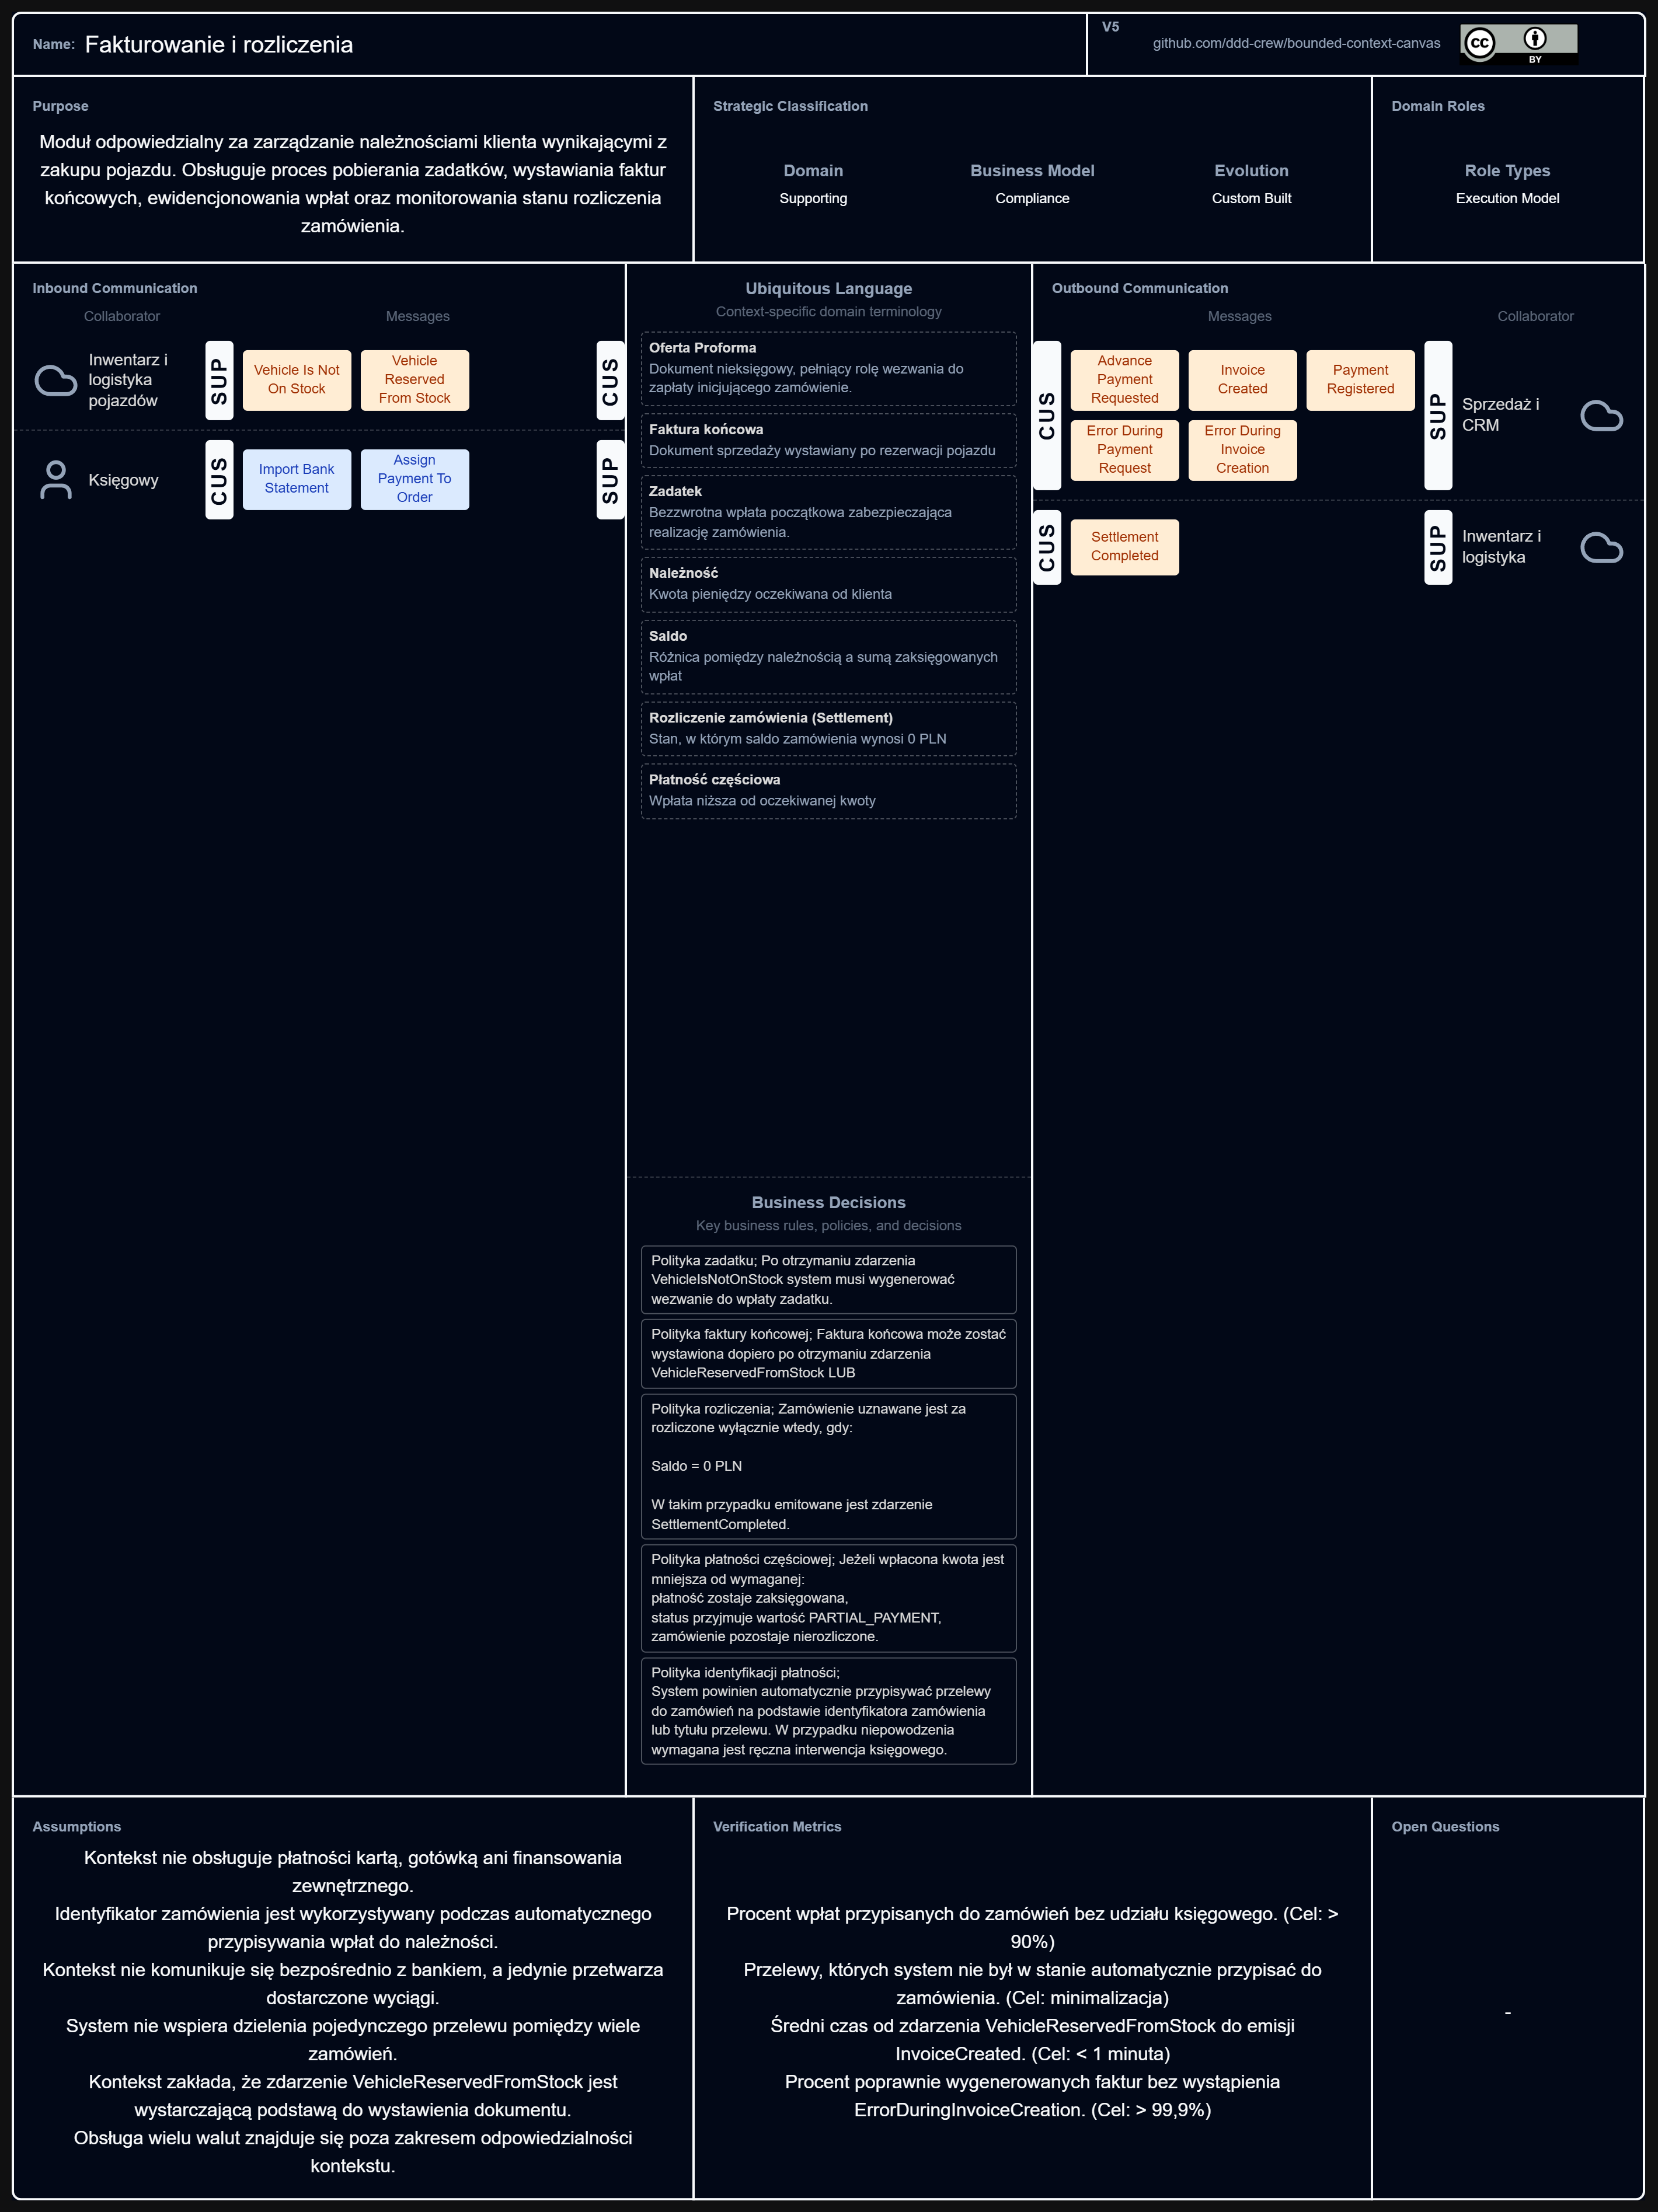
\includegraphics[width=0.9\textwidth]{media/bounded-context-canvas/final/FIR_K7_TOTAL_FINAL.png}
    \caption{Kanwa Kontekstu Fakturowania i Rozliczeń}
    \label{fig:hex_billing}
\end{figure}


\subsubsection{Przypadki użycia Kontekstu Fakturowania i Rozliczeń}

% =====================================================
\textbf{UC-FIR-01: Wysłanie prośby o zadatek}

\begin{longtable}{|p{4cm}|p{11cm}|}
\hline
\textbf{Element} & \textbf{Opis} \\
\hline

Identyfikator & UC-FIR-01 \\
\hline

Nazwa & Wysłanie prośby o zadatek \\
\hline

Opis & 
Przygotowanie danych do przelewu i powiadomienie klienta o konieczności wpłaty zadatku w przypadku braku pojazdu na placu. \\
\hline

Aktor główny & System (Kontekst Fakturowania) \\
\hline

Aktorzy pomocniczy & Klient \\
\hline

Warunki wstępne & 
Kontekst otrzymał zdarzenie \textit{VehicleIsNotOnStock}. \\
\hline

Warunki końcowe & 
Klient został poinformowany o wymaganej wpłacie, emitowane zdarzenie \textit{AdvancePaymentRequested}. \\
\hline

Scenariusz główny & 
\begin{enumerate}
    \item Kontekst fakturowania reaguje na zdarzenie \textit{VehicleIsNotOnStock}.
    \item System generuje numer rachunku bankowego oraz kwotę zadatku dla zamówienia.
    \item System wysyła do klienta informację (np. e-mail) z danymi do przelewu.
    \item Kontekst emituje zdarzenie \textit{AdvancePaymentRequested}.
\end{enumerate} \\
\hline

Scenariusze alternatywne & 
\begin{itemize}
    \item [A1] Błąd danych: Brak wymaganych informacji do wygenerowania prośby, system emituje \textit{ErrorDuringPaymentRequest}.
\end{itemize} \\
\hline
\end{longtable}

\begin{figure}[H]
    \centering
    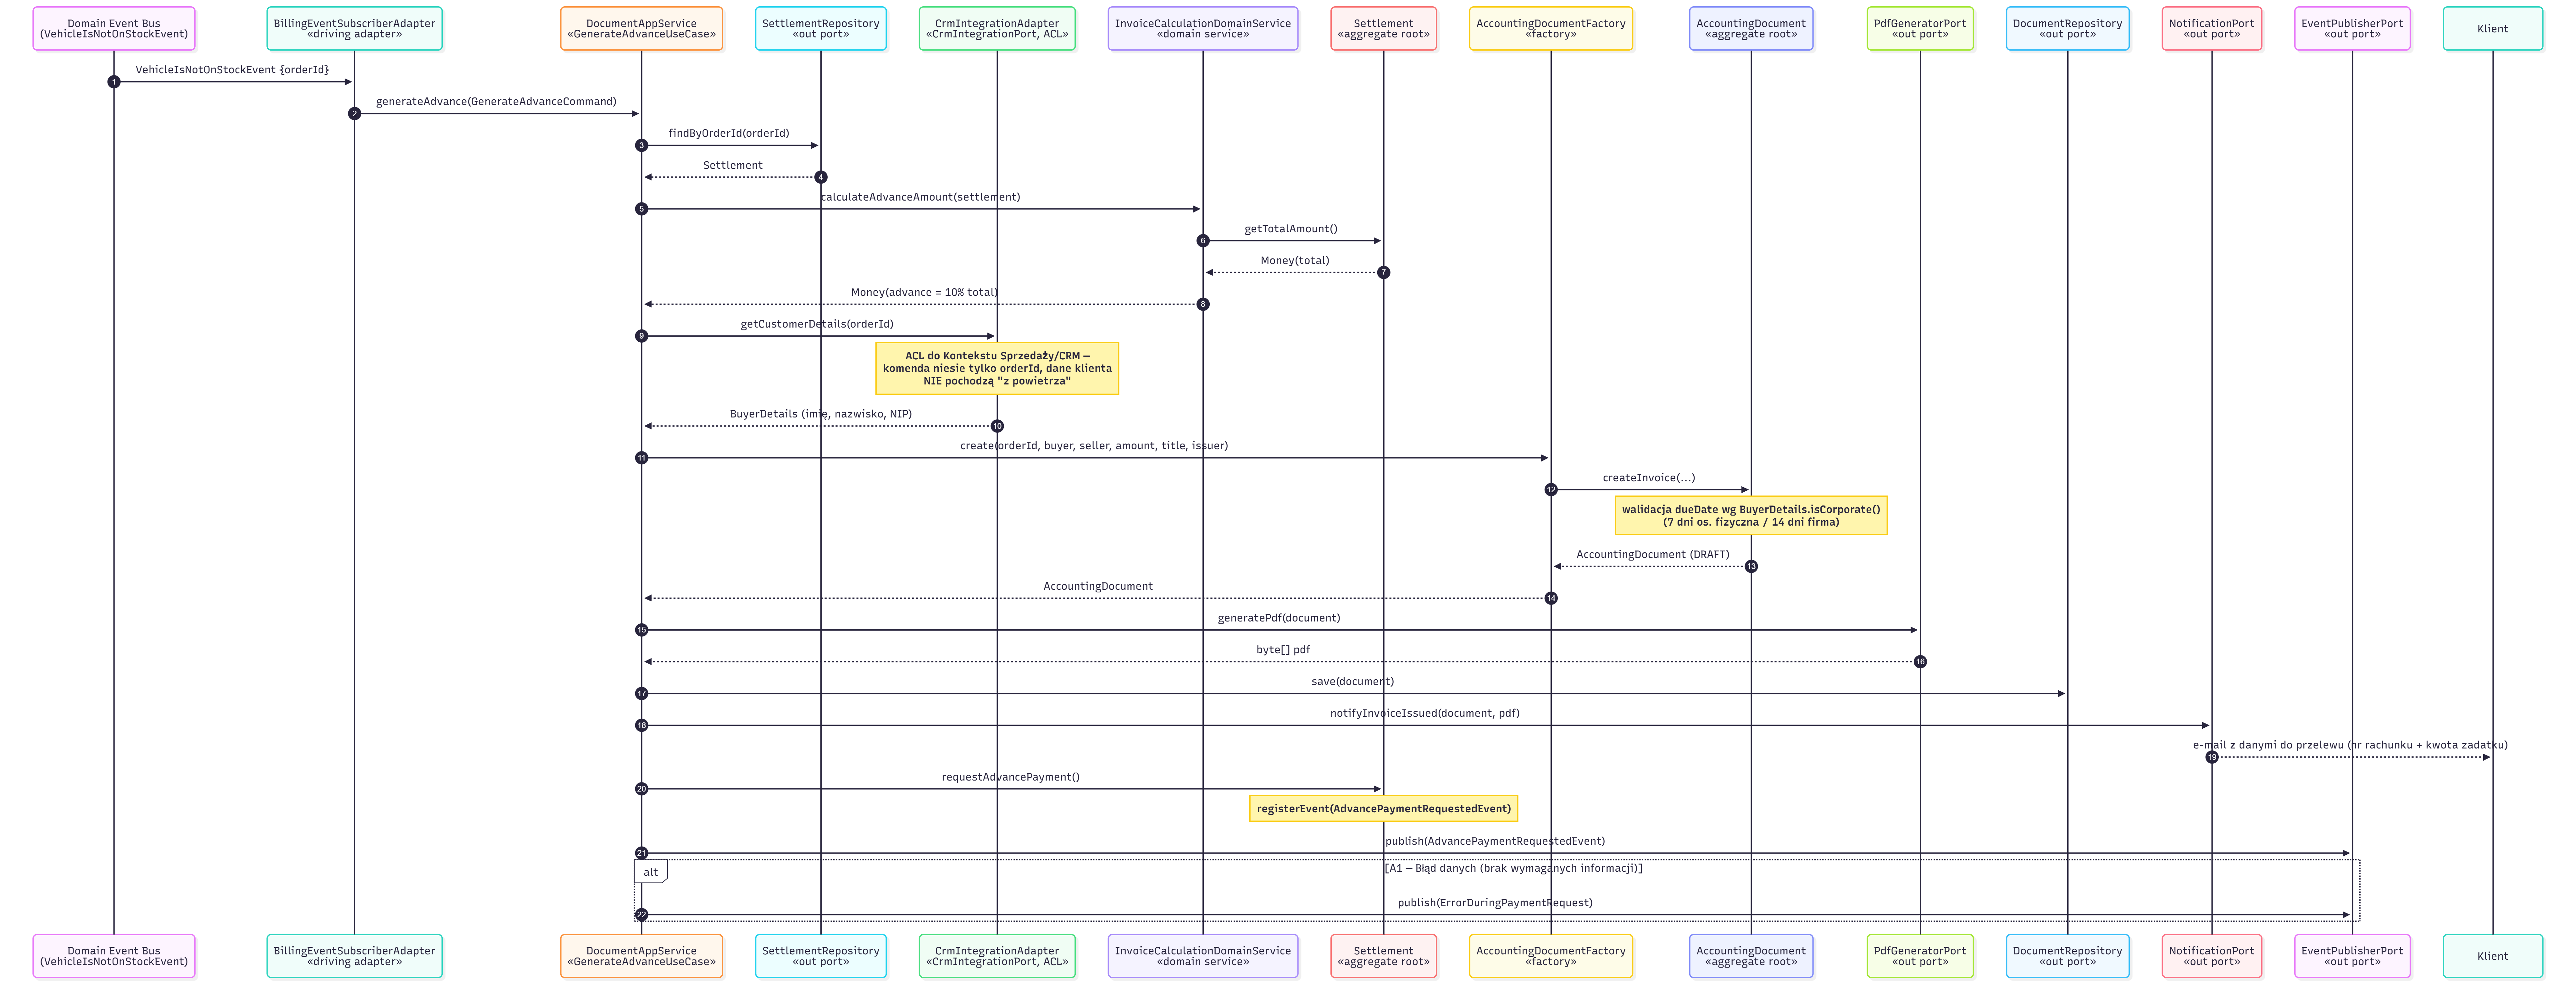
\includegraphics[width=1\textwidth]{media/diagramy_sekwencji/kontekst-faktur-rozliczenia/UC-FIR-01-Sekwencji.png}
    \caption{Diagram sekwencji dla przypadku użycia UC-FIR-01: Wysłanie prośby o zadatek}
    \label{fig:seq_uc_fir_01}
\end{figure}

% =====================================================
\textbf{UC-FIR-02: Stworzenie faktury końcowej}

\begin{longtable}{|p{4cm}|p{11cm}|}
\hline
\textbf{Element} & \textbf{Opis} \\
\hline

Identyfikator & UC-FIR-02 \\
\hline

Nazwa & Stworzenie faktury końcowej \\
\hline

Opis & 
Automatyczne wystawienie faktury końcowej po potwierdzeniu rezerwacji pojazdu z placu. \\
\hline

Aktor główny & System (Kontekst Fakturowania) \\
\hline

Aktorzy pomocniczy & - \\
\hline

Warunki wstępne & 
Kontekst otrzymał zdarzenie \textit{VehicleReservedFromStock}. \\
\hline

Warunki końcowe & 
Faktura PDF utworzona i przypisana do zamówienia, emitowane zdarzenie \textit{InvoiceCreated}. \\
\hline

Scenariusz główny & 
\begin{enumerate}
    \item Kontekst fakturowania reaguje na zdarzenie \textit{VehicleReservedFromStock}.
    \item System tworzy fakturę na kwotę pozostałą do zapłaty (uwzględniając ewentualne wpłaty zadatku).
    \item System wysyła do klienta informację (np. e-mail) z danymi do przelewu.
    \item System generuje plik PDF faktury i przypisuje go do zamówienia.
    \item Kontekst emituje zdarzenie \textit{InvoiceCreated}.
\end{enumerate} \\
\hline

Scenariusze alternatywne & 
\begin{itemize}
    \item [A1] Błąd generowania dokumentu: System nie może utworzyć pliku, emituje \textit{ErrorDuringInvoiceCreation}.
\end{itemize} \\
\hline
\end{longtable}

\begin{figure}[H]
    \centering
    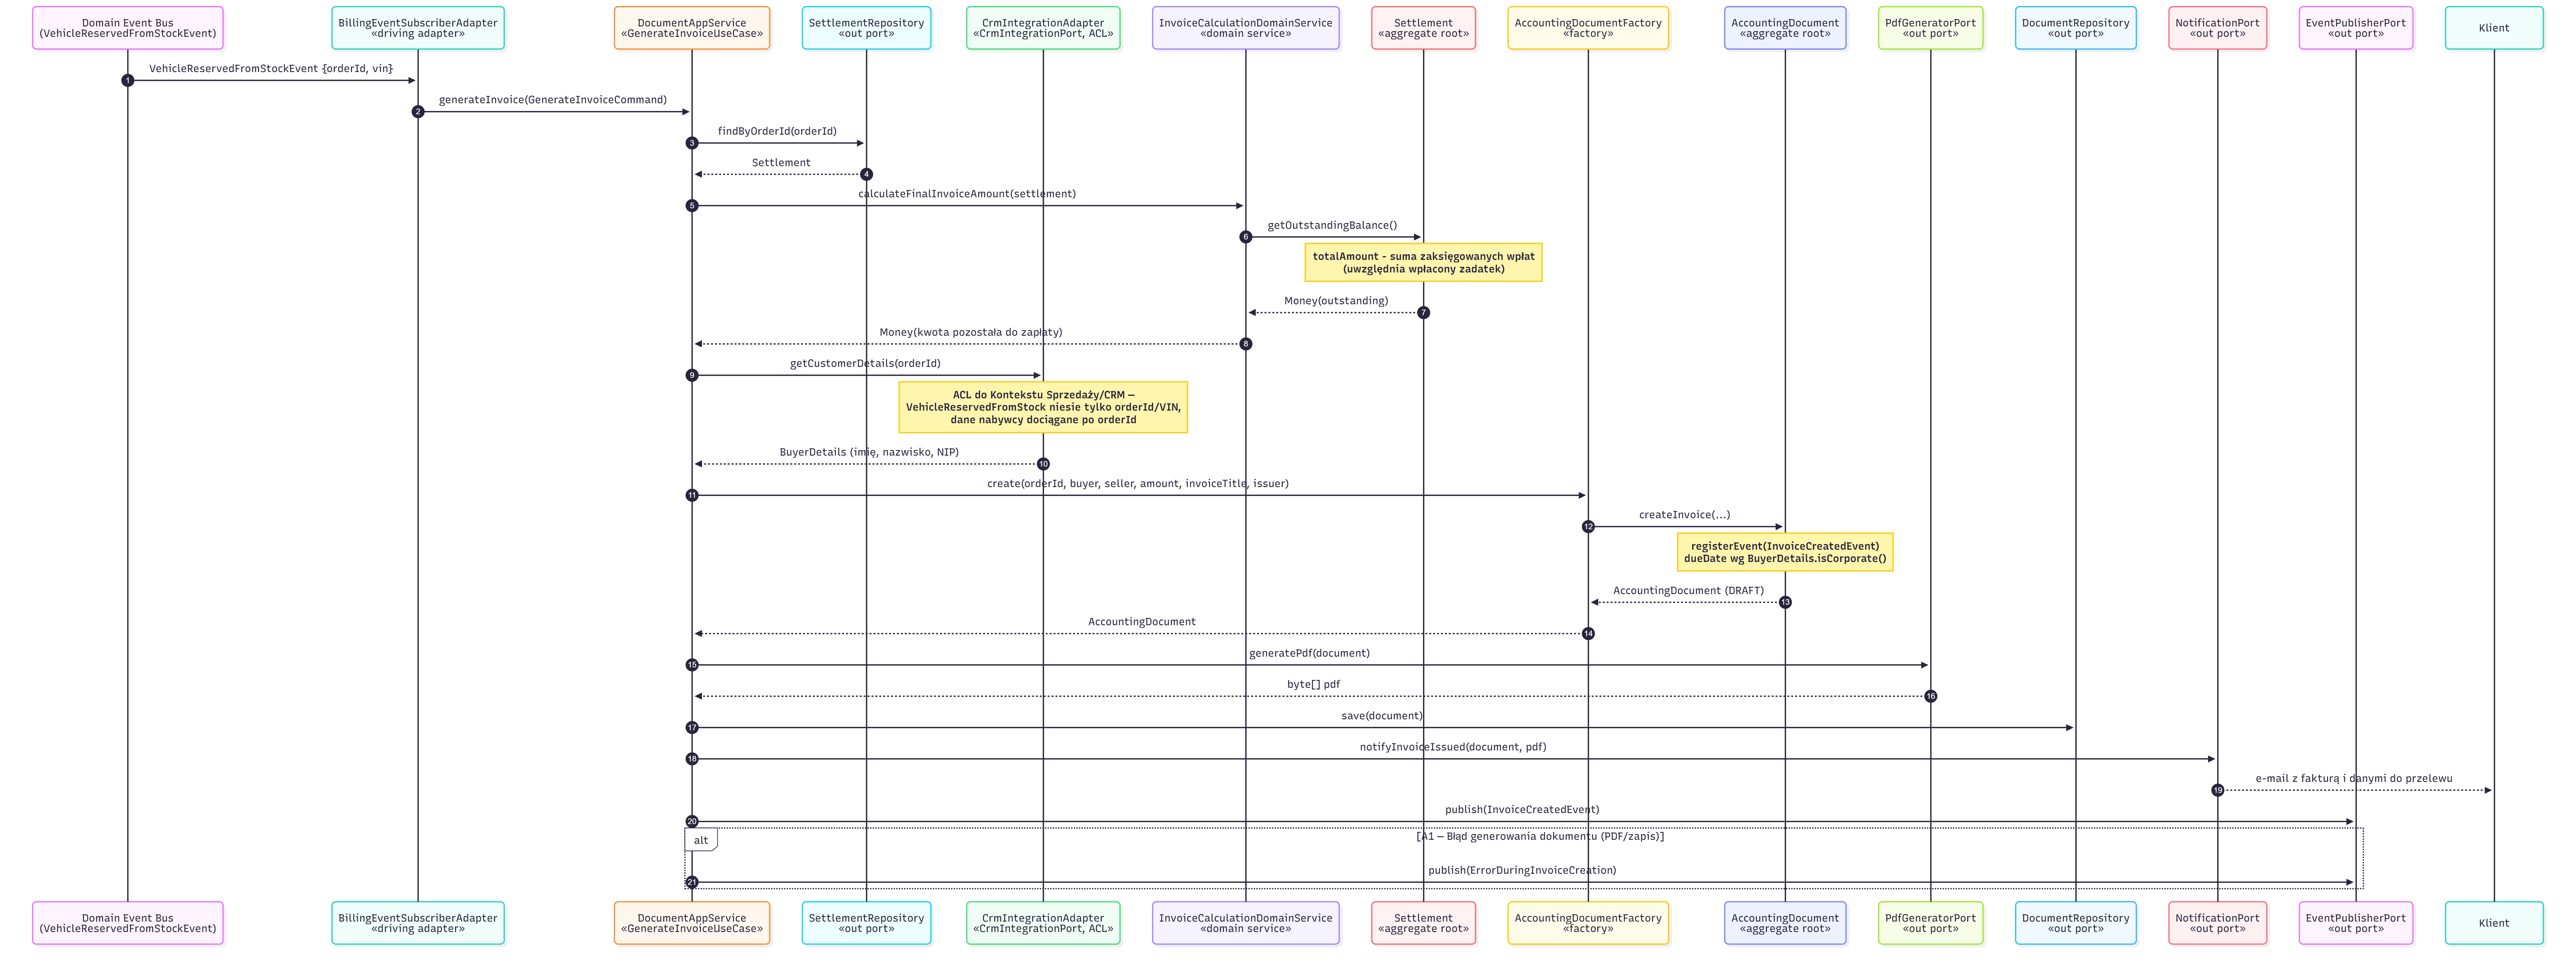
\includegraphics[width=1\textwidth]{media/diagramy_sekwencji/kontekst-faktur-rozliczenia/UC-FIR-02-Sekwencji.png}
    \caption{Diagram sekwencji dla przypadku użycia UC-FIR-02: Stworzenie faktury końcowe}
    \label{fig:seq_uc_fir_02}
\end{figure}

% =====================================================
\textbf{UC-FIR-03: Procesowanie płatności}

\begin{longtable}{|p{4cm}|p{11cm}|}
\hline
\textbf{Element} & \textbf{Opis} \\
\hline

Identyfikator & UC-FIR-03 \\
\hline

Nazwa & Procesowanie płatności \\
\hline

Opis & 
Zaksięgowanie przelewu bankowego i rozliczenie salda zamówienia. \\
\hline

Aktor główny & Księgowy \\
\hline

Aktorzy pomocniczy & System fakturowania \\
\hline

Warunki wstępne & 
W lokalnej bazie istnieje otwarta należność, księgowy zidentyfikował wpłatę na wyciągu. \\
\hline

Warunki końcowe & 
Płatność zarejestrowana, saldo zamówienia zaktualizowane, emitowane \textit{PaymentRegistered} (ewent. \textit{SettlementCompleted}). \\
\hline

Scenariusz główny & 
\begin{enumerate}
    \item Księgowy importuje plik wyciągu bankowego do systemu.
    \item System paruje przelew z zamówieniem (po tytule/ID). W przypadku braku dopasowania automatycznego, księgowy dokonuje weryfikacji ręcznej.
    \item System aktualizuje status płatności na 'SETTLED'.
    \item Kontekst emituje zdarzenie \textit{PaymentRegistered}.
    \item System weryfikuje sumę wpłat. Jeśli saldo = 0 PLN, kontekst emituje \textit{SettlementCompleted}.
\end{enumerate} \\
\hline

Scenariusze alternatywne & 
\begin{itemize}
    \item [A1] Błędna kwota: Kwota wpłaty różni się od wymaganej, system księguje częściowo, status płatności to \textit{PARTIAL\_PAYMENT}.
\end{itemize} \\
\hline
\end{longtable}

\begin{figure}[H]
    \centering
    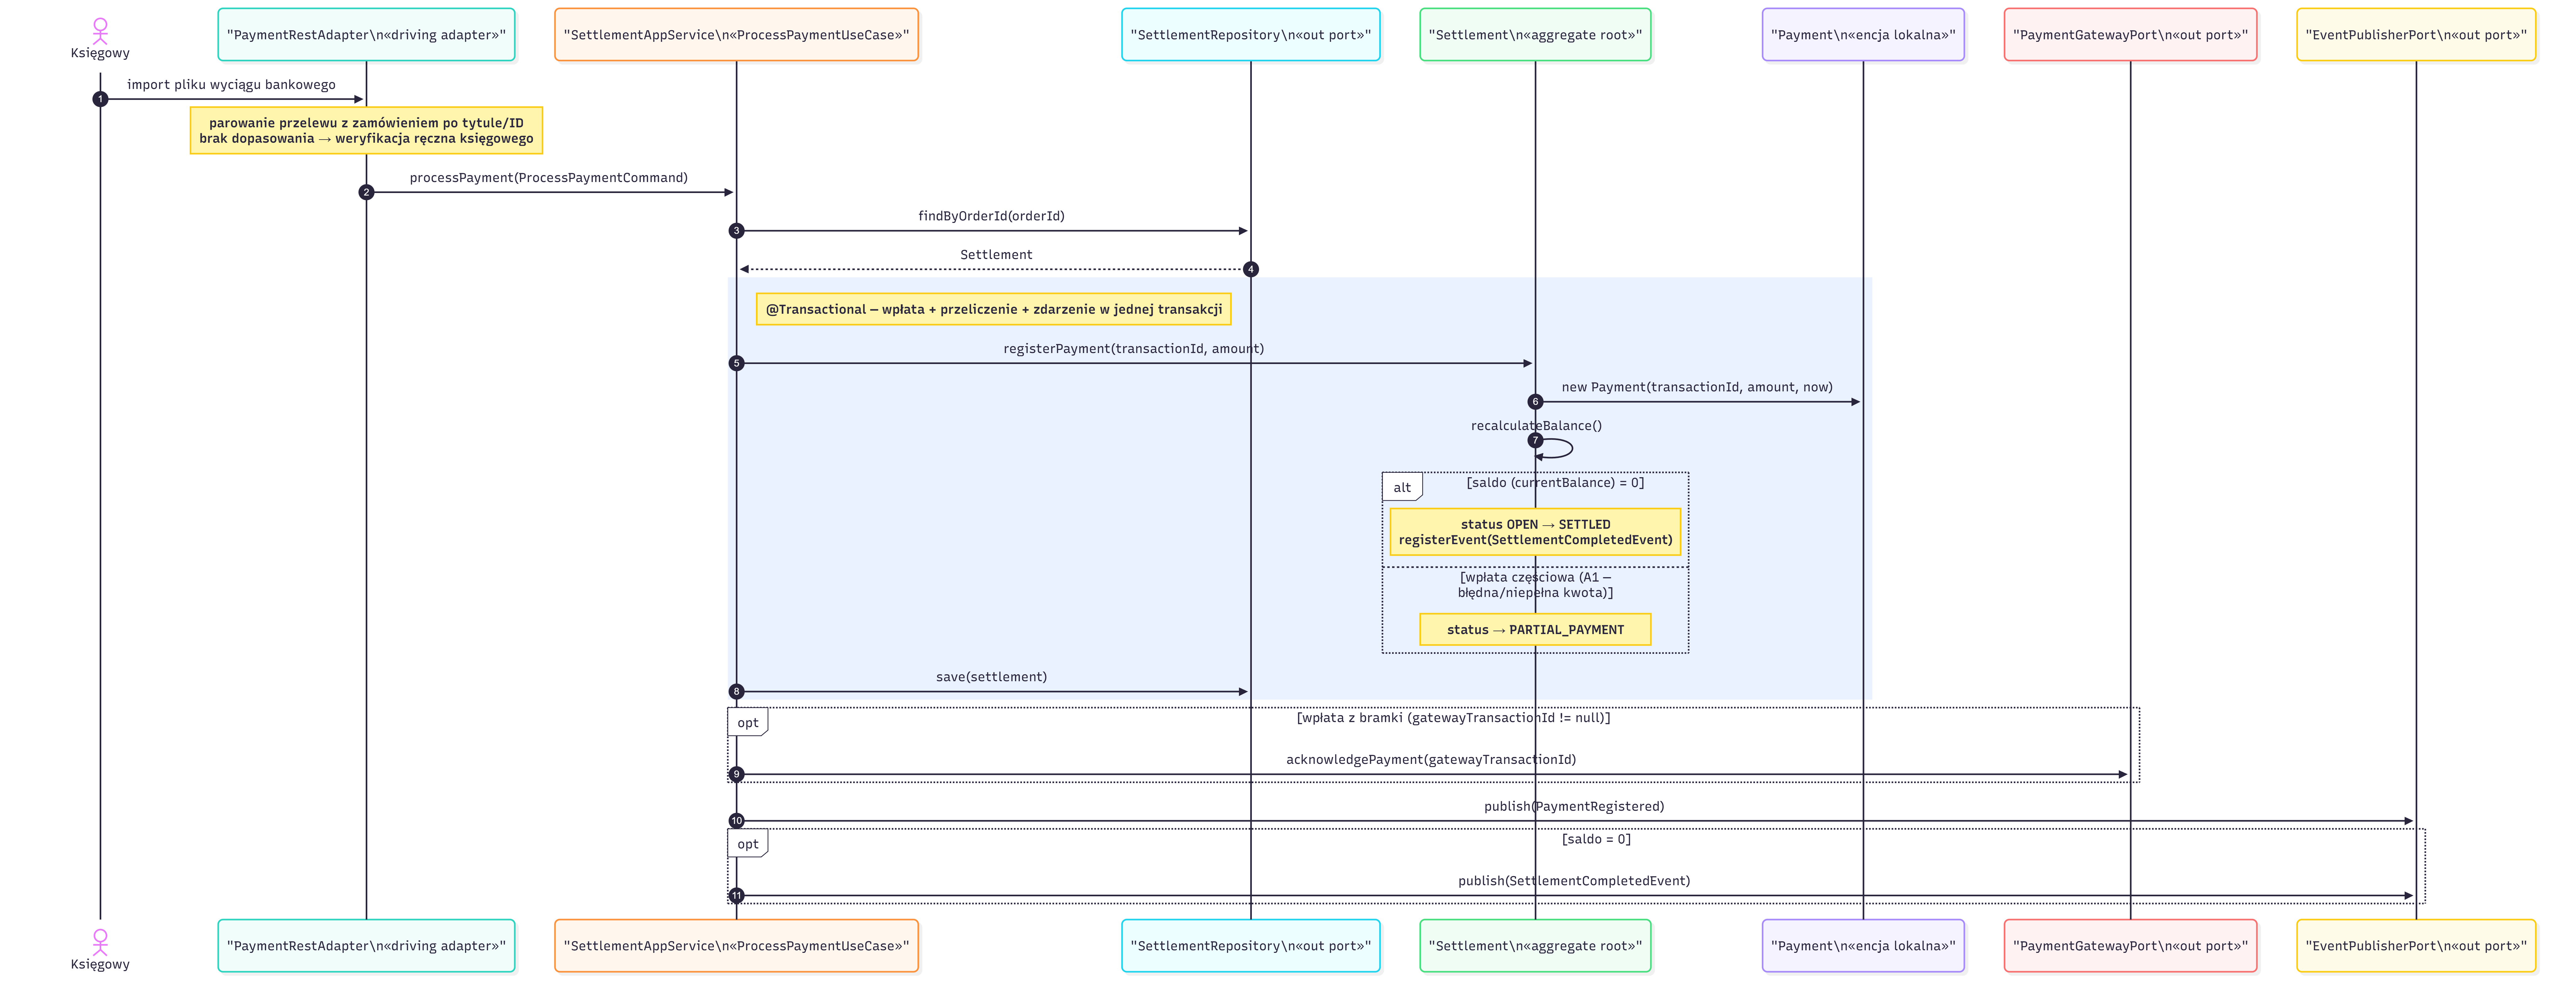
\includegraphics[width=1\textwidth]{media/diagramy_sekwencji/kontekst-faktur-rozliczenia/UC-FIR-03-Sekwencji.png}
    \caption{Diagram sekwencji dla przypadku użycia UC-FIR-03: Procesowanie płatności}
    \label{fig:seq_uc_fir_03}
\end{figure}

\subsubsection{Architektura Kontekstu Fakturowania i Rozliczeń}

Kontekst Fakturowania i Rozliczeń został zaprojektowany w oparciu o architekturę heksagonalną. Diagram Architektury przedstawiono na rysunku \ref{fig:hex_billing}.

\begin{figure}[H]
    \centering
    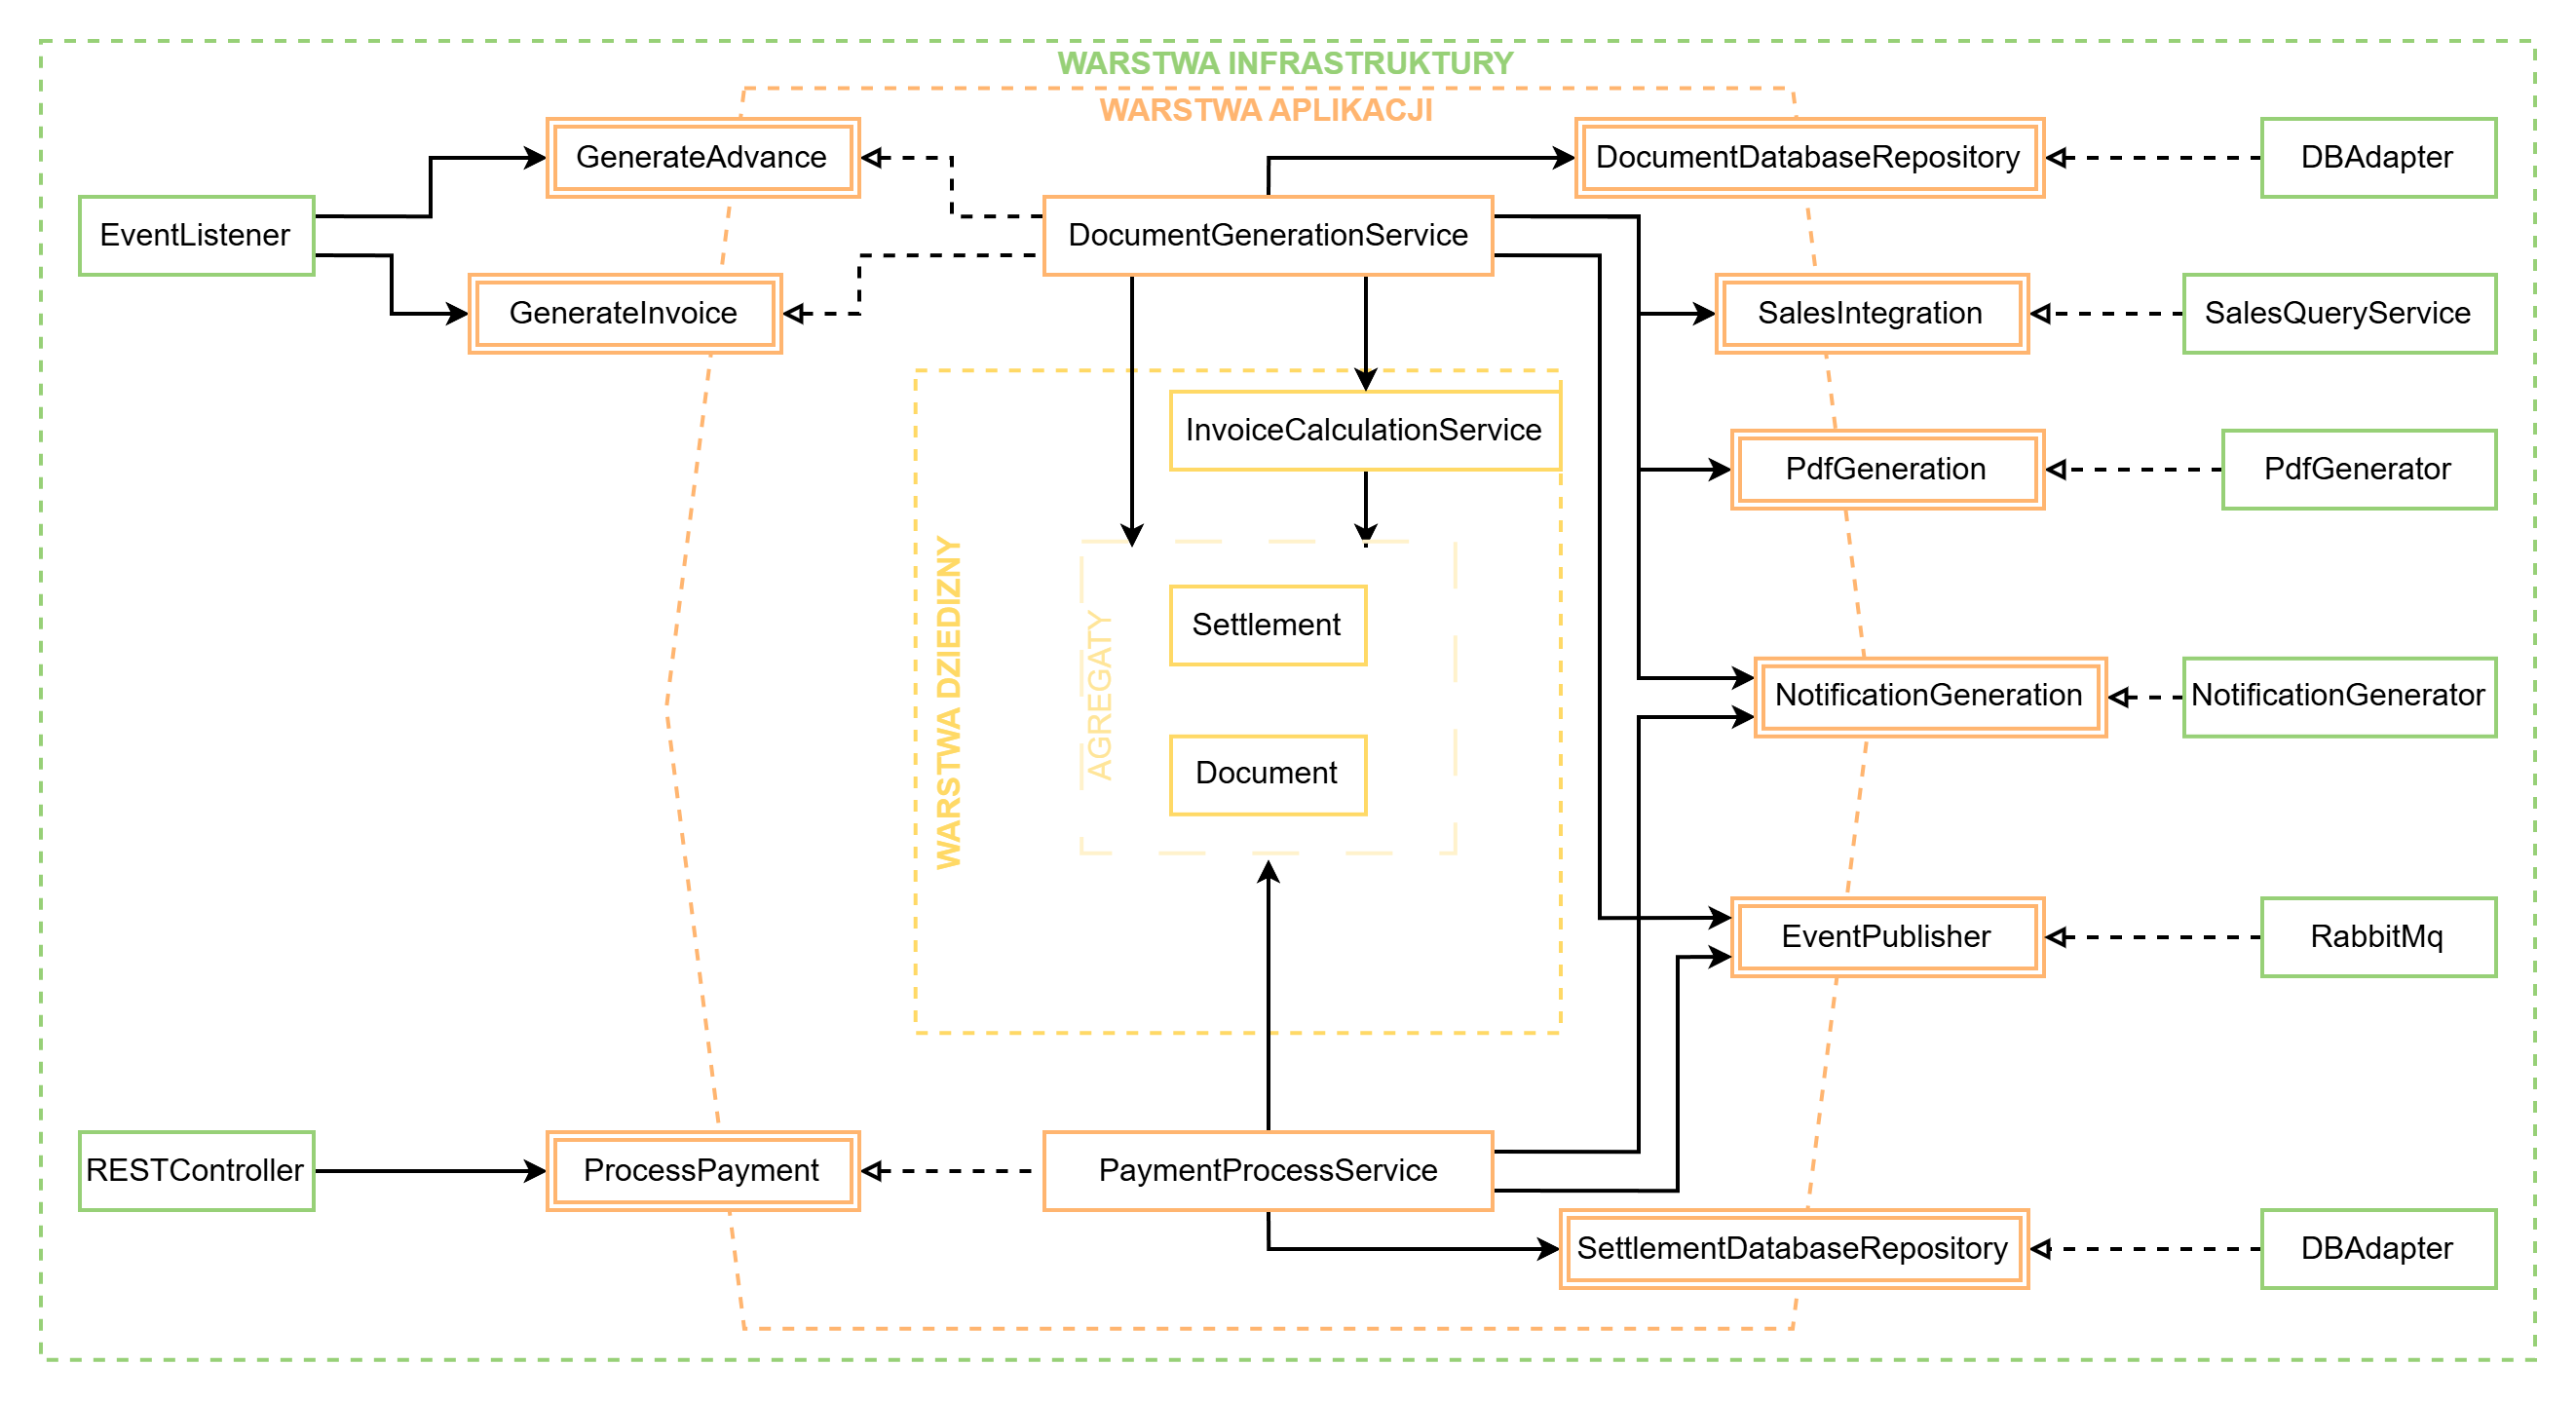
\includegraphics[width=1\linewidth]{media/architektura_heksagonalna/BillingArchitecture.png}
    \caption{Architektura heksagonalna kontekstu fakturowania i rozliczeń}
    \label{fig:hex_billing}
\end{figure}

Poniżej przedstawiono szczegółowy opis interakcji pomiędzy warstwami, z podziałem na strony wejściową i wyjściową.

\paragraph{Strona Wejściowa: Porty i Adaptery} 
Ta strona heksagonu definiuje, w jaki sposób świat zewnętrzny komunikuje się z Kontekstem Fakturowania w celu wyzwolenia konkretnych procesów biznesowych. Aby zachować spójność, interfejsy wejściowe zestawiono bezpośrednio z ich technicznymi implementacjami.

\begin{itemize}
    \item \textbf{Generowanie Dokumentów Finansowych (Asynchroniczne)}
    \begin{itemize}
        \item \textbf{Porty:} \texttt{GenerateAdvance} (wystawienie prośby o zadatek, UC-FIR-01) oraz \texttt{GenerateInvoice} (wystawienie faktury końcowej, UC-FIR-02). Oba interfejsy realizowane są przez jedną usługę aplikacyjną \texttt{DocumentGenerationService}.
        \item \textbf{Adapter:} \texttt{BillingEventSubscriberAdapter} (Messaging Adapter). Nasłuchuje na globalnej magistrali zdarzeń i przechwytuje zdarzenia logistyczne z Inwentarza (odpowiednio: \texttt{VehicleIsNotOnStock} oraz \texttt{VehicleReservedFromStock}), tłumaczy je na komendy (\texttt{GenerateAdvanceCommand}/\texttt{GenerateInvoiceCommand}) i asynchronicznie wyzwala powyższe porty.
    \end{itemize}

    \item \textbf{Zarządzanie Saldem i Wpłatami}
    \begin{itemize}
        \item \textbf{Port:} \texttt{ProcessPayment}. Interfejs obsługujący cykl życia salda (inicjalizacja, zaksięgowanie przelewu — UC-FIR-03 — oraz przypomnienia o płatności), realizowany przez \texttt{PaymentProcessService}.
        \item \textbf{Adaptery:} \texttt{SettlementEventListener} (Messaging Adapter) — nasłuchuje zdarzenia \texttt{OrderReadyForSettlement} z Kontekstu Sprzedaży i inicjalizuje saldo (\texttt{initializeSettlement}), realizując deduplikację po identyfikatorze zdarzenia; oraz \texttt{PaymentReminderCronJobAdapter} (Scheduling Adapter) — cyklicznie wyzwala wysyłkę przypomnień o niezapłaconych saldach (\texttt{sendPaymentReminders}). Ręczne zaksięgowanie wyciągu bankowego (\texttt{processPayment}, węzeł \texttt{RESTController} na diagramie) jest w obecnej implementacji obsługiwane przez warstwę aplikacji i pokryte testami; dedykowany adapter HTTP nie został jeszcze zaimplementowany.
    \end{itemize}
\end{itemize}

\paragraph{Strona Wyjściowa: Porty i Adaptery} 
Ta strona heksagonu definiuje, czego aplikacja potrzebuje od bazy danych, innych systemów, czy zewnętrznych bibliotek, aby zrealizować swoje zadanie.

\begin{itemize}
    \item \textbf{Utrwalanie Stanu (Persystencja)}
    \begin{itemize}
        \item \textbf{Porty:} \texttt{SettlementDatabaseRepository} oraz \texttt{DocumentDatabaseRepository}. Umożliwiają zapis i odczyt agregatów (\texttt{Settlement}, \texttt{AccountingDocument}), indeksowanych po \texttt{OrderId}.
        \item \textbf{Adaptery:} \texttt{InMemorySettlementRepository} oraz \texttt{InMemoryDocumentRepository} (węzeł \texttt{DBAdapter} na diagramie). W bieżącej implementacji są to atrapy przechowujące agregaty w pamięci (typu trwały magazyn); docelowo zostaną zastąpione adapterem bazodanowym (ORM/Hibernate) bez zmiany kontraktu portów.
    \end{itemize}

    \item \textbf{Integracja Międzykontekstowa (Anti-Corruption Layer)}
    \begin{itemize}
        \item \textbf{Port:} \texttt{SalesIntegration}. Query Port służący do synchronicznego dociągania danych nabywcy na podstawie \texttt{OrderId}.
        \item \textbf{Adapter:} \texttt{SalesCrmIntegrationAdapter}. Zależy wyłącznie od publicznej fasady Sprzedaży (\texttt{SalesQueryFacade}, Język Opublikowany), odbiera migawkę \texttt{CustomerSnapshotDto} i tłumaczy ją na hermetyczny obiekt wartości \texttt{BuyerDetails}, chroniąc domenę fakturowania przed korupcją obcymi modelami.
    \end{itemize}

    \item \textbf{Generowanie Plików i Powiadomienia}
    \begin{itemize}
        \item \textbf{Porty:} \texttt{PdfGeneration} oraz \texttt{NotificationGeneration}. Interfejsy zlecające odpowiednio wygenerowanie pliku PDF oraz wysyłkę wiadomości do klienta.
        \item \textbf{Adaptery:} \texttt{PdfGeneratorMockAdapter} (deleguje do metody \texttt{generatePdf()} agregatu \texttt{AccountingDocument}; docelowo wrapper na bibliotekę np. iText/PDFBox) oraz \texttt{NotificationAdapter}/\texttt{NotificationMockAdapter} (atrapy powiadomień konsolowych; docelowo wysyłka e-mail przez serwer SMTP).
    \end{itemize}

    \item \textbf{Publikacja Zdarzeń (Event Driven)}
    \begin{itemize}
        \item \textbf{Port:} \texttt{EventPublisher} (port Wspólnego Jądra). Umożliwia publikację zdarzeń wynikowych na magistralę.
        \item \textbf{Adapter:} \texttt{RabbitMqEventPublisherAdapter} (Wspólne Jądro) w uruchomieniu produkcyjnym lub \texttt{InProcessEventPublisherAdapter} (atrapa w procesie) w demach i testach. Odpowiada za serializację zdarzeń dziedzinowych (np. \texttt{InvoiceCreatedEvent}, \texttt{SettlementCompletedEvent}) i wysłanie ich na magistralę, domykając cykl komunikacji asynchronicznej.
    \end{itemize}
\end{itemize}

\paragraph{Usługi Aplikacji} 
Dla kontekstu Fakturowania i Rozliczeń, jako główne elementy orkiestrujące przepływ między portami wejściowymi a wyjściowymi, przewidziano:
\begin{itemize}
    \item \textbf{DocumentGenerationService} – realizuje orkiestrację dla UC-FIR-01 i UC-FIR-02. Pobiera dane o kliencie przez port CRM, wywołuje fabrykę dokumentów, zleca generowanie pliku PDF, notyfikuje użytkownika, zapisuje agregat \texttt{AccountingDocument} w bazie i emituje odpowiednie zdarzenia.
    \item \textbf{PaymentProcessService} – realizuje orkiestrację dla UC-FIR-03 w celu przetworzenia wpłaty klienta. Pobiera odpowiedni agregat \texttt{Settlement}, przekazuje mu parametry przelewu i publikuje zdarzenia.
\end{itemize}

\paragraph{Usługi Domenowe} 
Dla kontekstu Fakturowania i Rozliczeń, w celu ochrony czystości usług aplikacyjnych, wyodrębniono:
\begin{itemize}
    \item \textbf{InvoiceCalculationService} – bezstanowy serwis hermetyzujący zaawansowaną matematykę finansową. Zamyka w sobie logikę obliczania wysokości wymaganego zadatku (dla UC-FIR-01) oraz wyliczania ostatecznego salda pozostałego do zapłaty na fakturze końcowej (po uwzględnieniu historycznych wpłat dla UC-FIR-02).
\end{itemize}

% Poniżej przedstawiono szczegółowy opis interakcji pomiędzy warstwami oraz uzasadnienie wysoce izolowanego modelu modelowania taktycznego.

% \paragraph{Zarządzanie Wpłatami UC-FIR-03:}
% Ten segment systemu odpowiada za matematykę finansową i ewidencję wpłat. Zaprojektowano go tak, aby zagwarantować pełną spójność transakcyjną.
% \begin{itemize}
%     \item \textbf{Inicjalizacja:} Złożenie nowego zamówienia wyzwala port wejściowy, który poprzez usługę \linebreak \texttt{SettlementAppService} oddelegowuje zadanie do \texttt{SettlementFactory}. Fabryka powołuje do życia agregat salda na podstawie zamówienia uzyskanego w zdarzeniu.
%     \item \textbf{Rejestracja wpłaty:} Kiedy księgowy wgrywa wyciąg bankowy, port \texttt{ProcessPaymentUseCase} wysyła żądanie do usługi aplikacyjnej. Usługa pobiera agregat \texttt{Settlement} z bazy i wywołuje na nim mutację stanu. Pojedyncza wpłata nie posiada własnego repozytorium – jest enkapsulowana i zapisywana jako element kolekcji wewnątrz agregatu. Gwarantuje to, że wyliczenie salda zerowego i ewentualna emisja zdarzenia \texttt{SettlementCompletedEvent} zachodzą zawsze w jednej, bezpiecznej transakcji bazodanowej.
% \end{itemize}

% \paragraph{Wystawianie Faktur UC-FIR-01 i UC-FIR-02:}
% Segment ten zarządza generowaniem prawnie wiążących dokumentów PDF zadatku oraz faktury końcowej. Osiągnięto tu pełną izolację logiki wyliczeniowej od infrastruktury.
% \begin{itemize}
%     \item \textbf{Czystość Usługi Aplikacyjnej i Pobieranie Danych:} \texttt{DocumentAppService} pełni wyłącznie rolę kierownika przepływu. Nie zawiera instrukcji warunkowych ani operacji matematycznych. Odpowiada za koordynację wywołań pomiędzy domeną a portami wyjściowymi – w tym za synchroniczne odpytanie zewnętrznego kontekstu Sprzedaży i CRM poprzez port wyjściowy \texttt{CrmIntegrationPort} w celu dociągnięcia pełnych danych teleadresowych nabywcy (\texttt{BuyerDetails}) przed przystąpieniem do kreacji dokumentu. Zapobiega to niespójnościom wynikającym z faktu, że zdarzenia logistyczne z placu nie zawierają w sobie wrażliwych danych osobowych klientów.
%     \item \textbf{InvoiceCalculationDomainService} Wprowadzenie tego bezstanowego serwisu chroni warstwę aplikacji przed wyciekiem reguł biznesowych. Ponieważ wyliczenie ostatecznej kwoty faktury wymaga odjęcia zaksięgowanych wpłat od wartości kontraktu, serwis domenowy w sposób kontrolowany uzyskuje informacje ze stanu agregatu \texttt{Settlement}. Wylicza on kwotę i zwraca czysty obiekt wartości. Rozwiązanie to drastycznie zwiększa testowalność skomplikowanej matematyki księgowej.
%     \item \textbf{Bezpieczna Fabryka Dokumentu:} Gotowa kwota obliczona przez serwis domenowy przekazywana jest przez orkiestratora do \texttt{AccountingDocumentFactory}. Fabryka ta, łącząc kalkulacje finansowe z pobranym wcześniej z portu obiektem \texttt{BuyerDetails}, zajmuje się walidacją terminów płatności i zwraca poprawny, w pełni zainicjalizowany agregat \texttt{AccountingDocument}.
% \end{itemize}

% \paragraph{Porty Wyjściowe i Zdarzenia:} Do realizacji powyższych celów potrzebne również są porty realizujące poniższe zadania:
% \begin{itemize}
%     \item \textbf{NotificationPort} i \textbf{PdfGeneratorPort}: Zamiast implementować biblioteki do obsługi protokołu SMTP czy generowania plików PDF bezpośrednio w logice aplikacji, zdefiniowano interfejsy. Konkretne adaptery zostaną wstrzyknięte w zewnętrznym pierścieniu infrastruktury.
%     \item \textbf{CrmIntegrationPort:} Międzykontekstowy port wyjściowy typu Query. Odpowiada za synchroniczne pobranie danych tożsamościowych i skarbowych klienta z modułu CRM na podstawie \texttt{OrderId}. Użycie dedykowanego portu zapewnia zgodność z regulacjami RODO, izolując dane osobowe od globalnej magistrali komunikatów logistycznych.
%     \item \textbf{Magistrala Zdarzeń (Domain Event Bus):} Przepływ pracy kończy się wyemitowaniem zdarzeń dziedzinowych (np. \texttt{AdvancePaymentRequested}, \texttt{InvoiceCreated}), co pozwala reszcie systemu (np. modułowi Sprzedaży) na asynchroniczne reagowanie bez tworzenia cyklicznych zależności.
% \end{itemize}

\subsubsection{Agregaty Kontekstu Fakturowania i Rozliczeń}

Model taktyczny tego kontekstu został zdekomponowany na dwa agregaty. Taki podział eliminuje ryzyko blokad bazy danych (np. podczas jednoczesnej rejestracji wpłaty przez bramkę online i wystawiania faktury przez księgowość).

\begin{figure}[H]
    \centering
    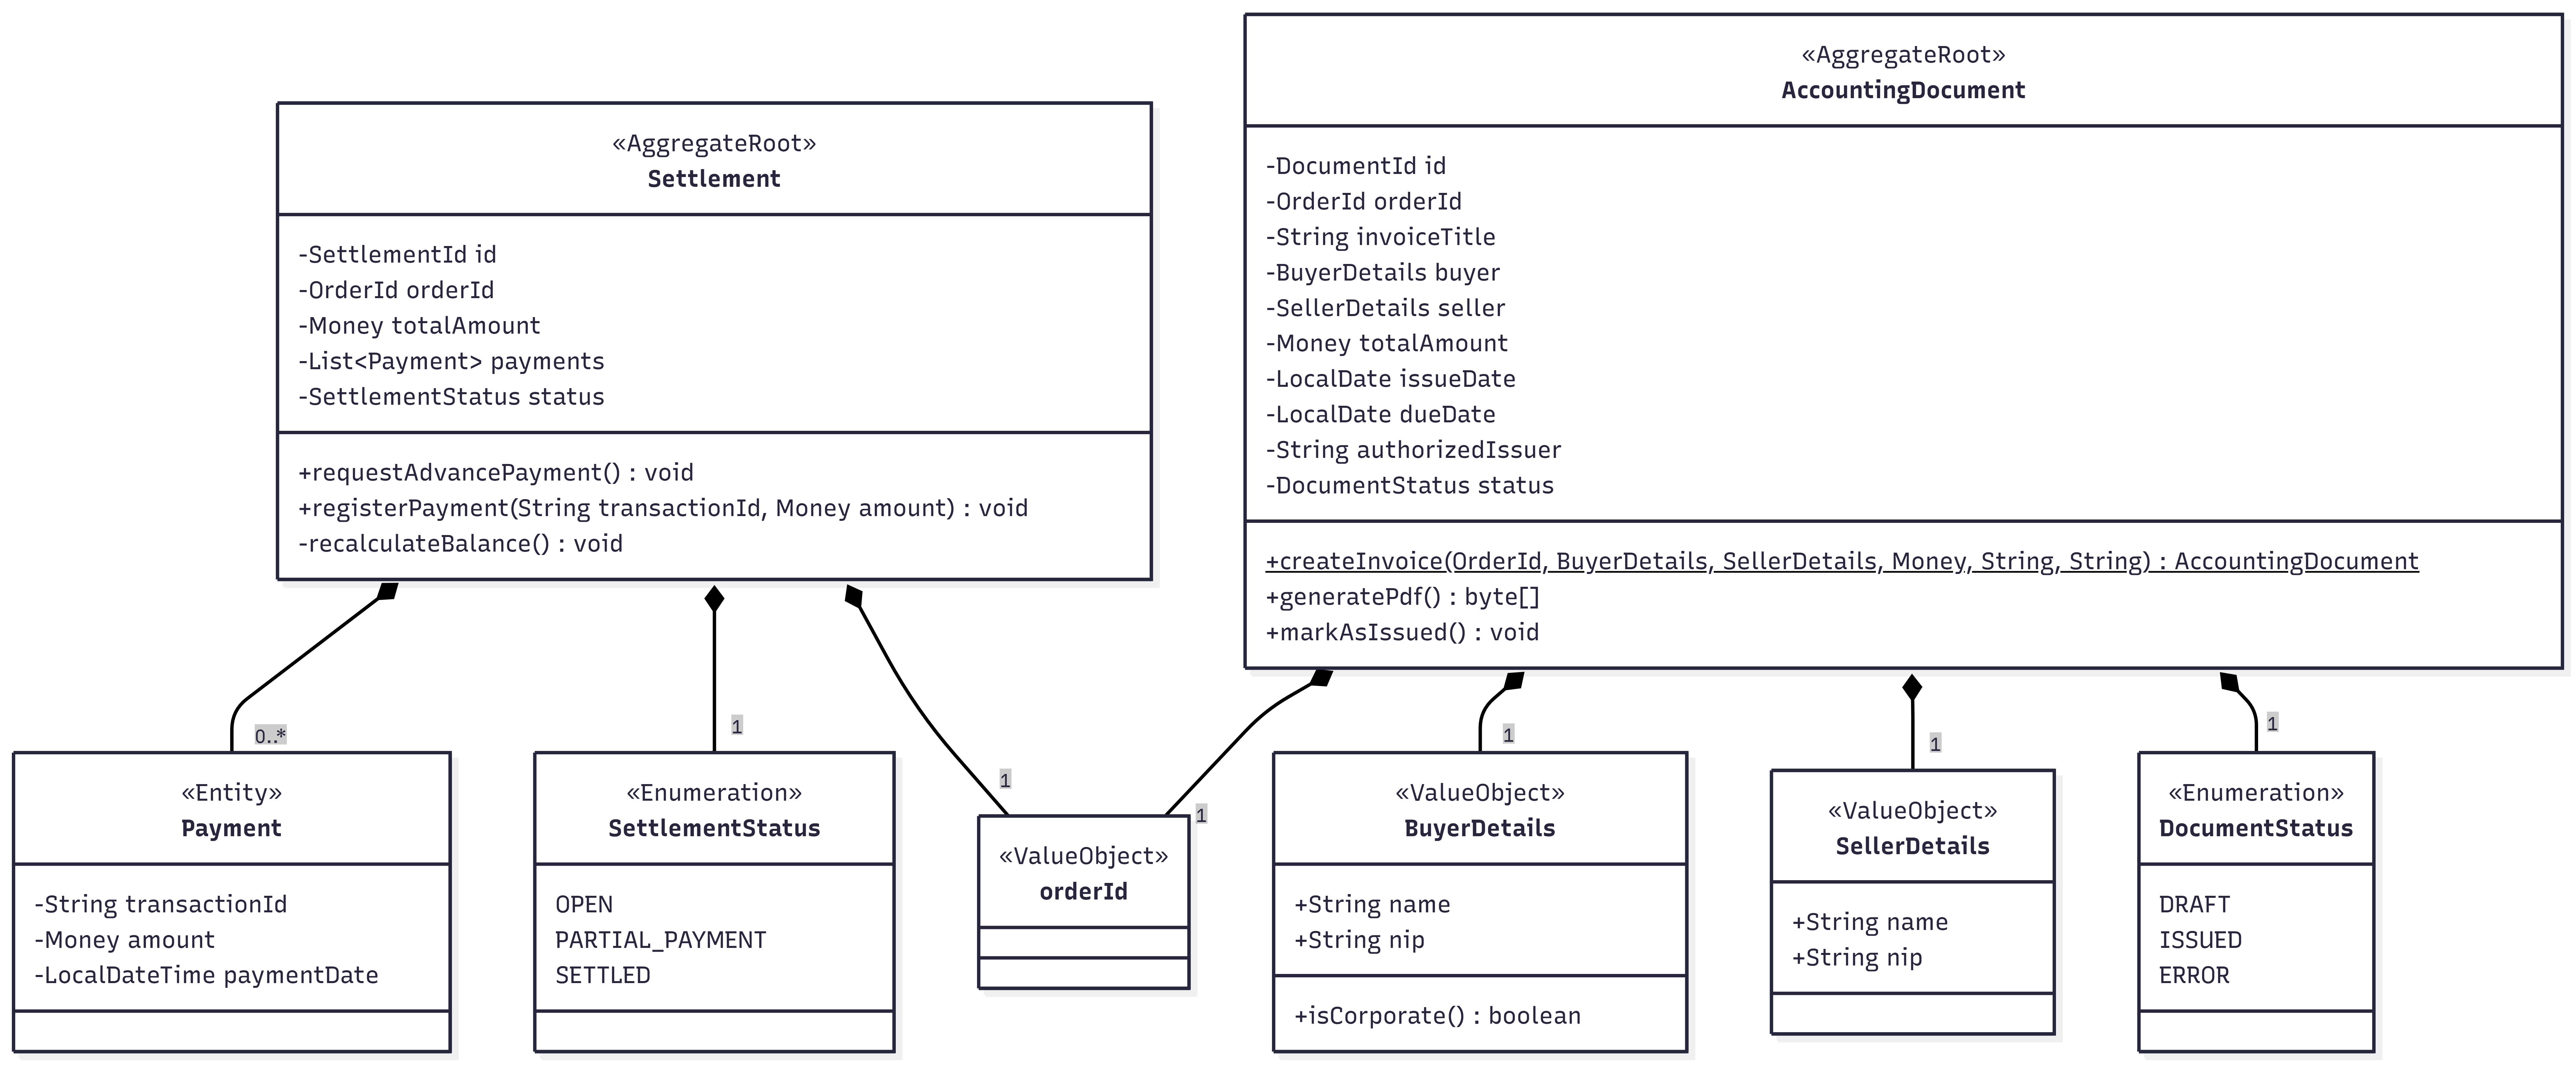
\includegraphics[width=\textwidth]{media/agregaty/kontekst-fakturowania-rozliczen/settlement-document.png}
    \caption{Model strukturalny agregatów kontekstu fakturowania i rozliczeń}
    \label{fig:agg_payment}
\end{figure}

Logika biznesowa została skondensowana wokół dwóch wysoce spójnych agregatów: \texttt{Settlement} oraz \texttt{AccountingDocument}.

\paragraph{Agregat: Settlement (Rozliczenie Zamówienia)}
Agregat ten stanowi centralny mechanizm kontroli finansowej dla konkretnego kontraktu, powiązany z nim poprzez niemutowalny identyfikator \texttt{OrderId}. Zgodnie z podziałem odpowiedzialności, jego wyłącznym zadaniem jest obsługa ewidencji wpłat (Przypadek użycia \textbf{UC-FIR-03}).
\begin{itemize}
    \item \textbf{Encja Lokalna Wpłaty (\texttt{Payment}):} Pojedyncze transakcje z wyciągów bankowych nie posiadają globalnej tożsamości. Są one traktowane jako encje lokalne wewnątrz agregatu \texttt{Settlement}. Gwarantuje to, że wpłata nie może istnieć w systemie w oderwaniu od przypisanego do niej zamówienia.
    \item \textbf{Ochrona Niezmienników:} Agregat jest wyłącznym właścicielem reguł matematycznych. Rejestracja nowej wpłaty (metoda \texttt{registerPayment}) powoduje dodanie jej do wewnętrznej kolekcji oraz natychmiastowe, ukryte przeliczenie pola \texttt{currentBalance} względem całkowitej wartości kontraktu \texttt{totalAmount} (wewnętrzna metoda \texttt{recalculateBalance}). 
    \item \textbf{Autonomiczna Zmiana Stanu:} Na podstawie wyliczonego bieżącego bilansu, agregat samodzielnie podejmuje decyzję o zmianie statusu z \texttt{OPEN} na \texttt{PARTIAL\_PAYMENT} lub \texttt{SETTLED}. Osiągnięcie zerowego zadłużenia (\texttt{currentBalance} = 0) skutkuje natychmiastową kreacją wewnątrz agregatu zdarzenia \texttt{SettlementCompletedEvent}, które zamyka proces rozliczenia.
\end{itemize}

\paragraph{Agregat: AccountingDocument (Dokument Księgowy)}
Agregat odpowiedzialny za procesowanie prawnie wiążących dokumentów skarbowych (zarówno Faktur Końcowych, jak i Proform). Przejęcie pełnej odpowiedzialności za oficjalną komunikację finansową sprawia, że wspiera on realizację aż dwóch przypadków użycia: \textbf{UC-FIR-01} (prośba o zadatek) oraz \textbf{UC-FIR-02} (faktura końcowa). Oddzielenie go od agr